%pdflatex abra.tex
%convert -density 150x150 abra.pdf abra.png
\documentclass[border={2pt 2pt 2pt 2pt}]{standalone}
\usepackage{tikz}
\usetikzlibrary{calc}
\begin{document}

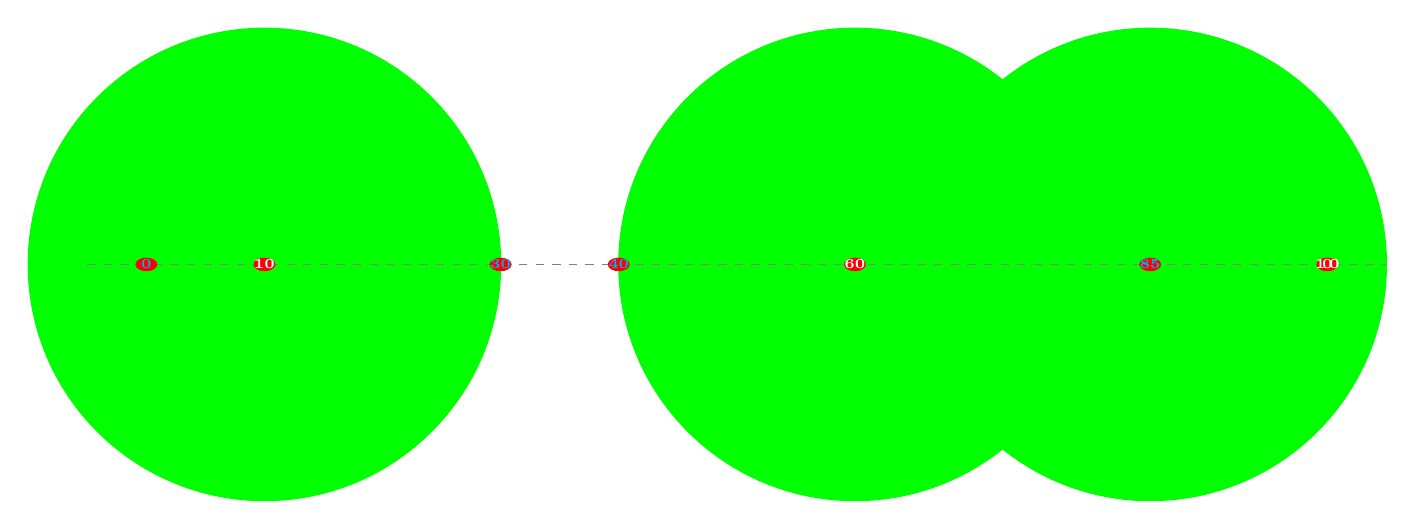
\begin{tikzpicture}[scale=0.15]
\coordinate (A) at (0,0);
\coordinate (B) at (10,0);
\coordinate (C) at (30,0);
\coordinate (D) at (40,0);
\coordinate (E) at (60,0);
\coordinate (F) at (85,0);
\coordinate (G) at (100,0);
\draw[green,fill=green] (B) circle [radius=20];
\draw[green,fill=green] (E) circle [radius=20];
\draw[green,fill=green] (F) circle [radius=20];
\draw[dashed,gray] (-5,0)--(105,0);
\draw[red,fill=red] (A) ellipse (25pt and 15pt);
\draw[red,fill=red] (B) ellipse (25pt and 15pt);
\draw[red,fill=red] (C) ellipse (25pt and 15pt);
\draw[red,fill=red] (D) ellipse (25pt and 15pt);
\draw[red,fill=red] (E) ellipse (25pt and 15pt);
\draw[red,fill=red] (F) ellipse (25pt and 15pt);
\draw[red,fill=red] (G) ellipse (25pt and 15pt);
\node[cyan] at (A) {\bf\tiny 0};
\node[white] at (B) {\bf\tiny 10};
\node[cyan] at (C) {\bf\tiny 30};
\node[cyan] at (D) {\bf\tiny 40};
\node[white] at (E) {\bf\tiny 60};
\node[cyan] at (F) {\bf\tiny 85};
\node[white] at (G) {\bf\tiny 1\!0\!0};
\end{tikzpicture}

\end{document}
